\documentclass[journal,12pt,twocolumn]{IEEEtran}

\usepackage{setspace}
\usepackage{gensymb}
\singlespacing
\usepackage[cmex10]{amsmath}

\usepackage{amsthm}

\usepackage{mathrsfs}
\usepackage{txfonts}
\usepackage{stfloats}
\usepackage{bm}
\usepackage{cite}
\usepackage{cases}
\usepackage{subfig}

\usepackage{longtable}
\usepackage{multirow}

\usepackage{enumitem}
\usepackage{mathtools}
\usepackage{steinmetz}
\usepackage{tikz}
\usepackage{circuitikz}
\usepackage{verbatim}
\usepackage{tfrupee}
\usepackage[breaklinks=true]{hyperref}
\usepackage{graphicx}
\usepackage{tkz-euclide}

\usetikzlibrary{calc,math}
\usepackage{listings}
    \usepackage{color}                                            %%
    \usepackage{array}                                            %%
    \usepackage{longtable}                                        %%
    \usepackage{calc}                                             %%
    \usepackage{multirow}                                         %%
    \usepackage{hhline}                                           %%
    \usepackage{ifthen}                                           %%
    \usepackage{lscape}     
\usepackage{multicol}
\usepackage{chngcntr}

\DeclareMathOperator*{\Res}{Res}

\renewcommand\thesection{\arabic{section}}
\renewcommand\thesubsection{\thesection.\arabic{subsection}}
\renewcommand\thesubsubsection{\thesubsection.\arabic{subsubsection}}

\renewcommand\thesectiondis{\arabic{section}}
\renewcommand\thesubsectiondis{\thesectiondis.\arabic{subsection}}
\renewcommand\thesubsubsectiondis{\thesubsectiondis.\arabic{subsubsection}}


\hyphenation{op-tical net-works semi-conduc-tor}
\def\inputGnumericTable{}                                 %%

\lstset{
%language=C,
frame=single, 
breaklines=true,
columns=fullflexible
}
\begin{document}

\newcommand{\BEQA}{\begin{eqnarray}}
\newcommand{\EEQA}{\end{eqnarray}}
\newcommand{\define}{\stackrel{\triangle}{=}}
\bibliographystyle{IEEEtran}
\raggedbottom
\setlength{\parindent}{0pt}
\providecommand{\mbf}{\mathbf}
\providecommand{\pr}[1]{\ensuremath{\Pr\left(#1\right)}}
\providecommand{\qfunc}[1]{\ensuremath{Q\left(#1\right)}}
\providecommand{\sbrak}[1]{\ensuremath{{}\left[#1\right]}}
\providecommand{\lsbrak}[1]{\ensuremath{{}\left[#1\right.}}
\providecommand{\rsbrak}[1]{\ensuremath{{}\left.#1\right]}}
\providecommand{\brak}[1]{\ensuremath{\left(#1\right)}}
\providecommand{\lbrak}[1]{\ensuremath{\left(#1\right.}}
\providecommand{\rbrak}[1]{\ensuremath{\left.#1\right)}}
\providecommand{\cbrak}[1]{\ensuremath{\left\{#1\right\}}}
\providecommand{\lcbrak}[1]{\ensuremath{\left\{#1\right.}}
\providecommand{\rcbrak}[1]{\ensuremath{\left.#1\right\}}}
\theoremstyle{remark}
\newtheorem{rem}{Remark}
\newcommand{\sgn}{\mathop{\mathrm{sgn}}}
\providecommand{\abs}[1]{\vert#1\vert}
\providecommand{\res}[1]{\Res\displaylimits_{#1}} 
\providecommand{\norm}[1]{\lVert#1\rVert}
%\providecommand{\norm}[1]{\lVert#1\rVert}
\providecommand{\mtx}[1]{\mathbf{#1}}
\providecommand{\mean}[1]{E[ #1 ]}
\providecommand{\fourier}{\overset{\mathcal{F}}{ \rightleftharpoons}}
%\providecommand{\hilbert}{\overset{\mathcal{H}}{ \rightleftharpoons}}
\providecommand{\system}{\overset{\mathcal{H}}{ \longleftrightarrow}}
	%\newcommand{\solution}[2]{\textbf{Solution:}{#1}}
\newcommand{\solution}{\noindent \textbf{Solution: }}
\newcommand{\cosec}{\,\text{cosec}\,}
\providecommand{\dec}[2]{\ensuremath{\overset{#1}{\underset{#2}{\gtrless}}}}
\providecommand{\gauss}[2]{\mathcal{N}\ensuremath{\left(#1,#2\right)}}
\newcommand{\myvec}[1]{\ensuremath{\begin{pmatrix}#1\end{pmatrix}}}
\newcommand{\mydet}[1]{\ensuremath{\begin{vmatrix}#1\end{vmatrix}}}
\numberwithin{equation}{subsection}
\makeatletter
\@addtoreset{figure}{problem}
\makeatother
\let\StandardTheFigure\thefigure
\let\vec\mathbf
\renewcommand{\thefigure}{\theproblem}
\def\putbox#1#2#3{\makebox[0in][l]{\makebox[#1][l]{}\raisebox{\baselineskip}[0in][0in]{\raisebox{#2}[0in][0in]{#3}}}}
     \def\rightbox#1{\makebox[0in][r]{#1}}
     \def\centbox#1{\makebox[0in]{#1}}
     \def\topbox#1{\raisebox{-\baselineskip}[0in][0in]{#1}}
     \def\midbox#1{\raisebox{-0.5\baselineskip}[0in][0in]{#1}}
\vspace{3cm}
\title{ 7.2,7.3}%number
\author{7.2,7.3}
\maketitle
\newpage
\bigskip
\renewcommand{\thefigure}{\theenumi}
\renewcommand{\thetable}{\theenumi}
\newcommand*{\permcomb}[4][0mu]{{{}^{#3}\mkern#1#2_{#4}}}
\newcommand*{\perm}[1][-3mu]{\permcomb[#1]{P}}
\newcommand*{\comb}[1][-1mu]{\permcomb[#1]{C}}
Download all python codes from 
\renewcommand{\theequation}{\theenumi}
\renewcommand{\thefigure}{\theenumi}

%\subsection{Independence}
\subsection{Using Definition}
\begin{enumerate}[label=\thesection.\arabic*.,ref=\thesection.\theenumi]
\numberwithin{equation}{enumi}
\numberwithin{figure}{enumi}
%%
\item
\label{ch4_sim}
Plot 
\begin{equation}
P_e = \pr{\hat{X} = -1|X=1}
\end{equation}
%
for 
\begin{equation}
Y = AX+N,
\end{equation}
where $A$ is Raleigh with $E\sbrak{A^2} = \gamma, N \sim \gauss{0}{1}, X \in \brak{-1,1}$ for $0 \le \gamma \le 10$ dB.

%
\item
Assuming that $N$ is a constant, find an expression for $P_e$.  Call this $P_e(N)$\\
\solution The estimated value $\hat{X}$ is given by
\begin{align}
\hat{X} = 
\begin{cases}
+1 & Y>0\\
-1 & Y<0
\end{cases}
\end{align}
For $X = 1$, 
\begin{align}
Y &= A + N\\
P_e &= \pr{\hat{X} = -1|X=1} \\
&= \pr{Y<0 |X=1}\\
&= \pr{A<-N}\\
&= F_A(-N)\\
&= \int_{-\infty}^{-N} f_A(x)dx
\end{align}
By definition
\begin{align}
f_A(x) = 
\begin{cases}
\frac{x}{\sigma^2}\exp\brak{{-\frac{x^2}{2\sigma^2}}} & x\geq0\\
0 & otherwise
\end{cases}
\end{align}
If $N>0, f_A(x) = 0$. Then,
\begin{align}
 P_e=0  
\end{align}
If $N<0$. Then,
\begin{align}
 P_e(N) &=\int_{-\infty}^{-N} f_A(x)dx\\
 &=\int_{-\infty}^{0} 0dx+\int_{0}^{-N} f_A(x)dx\\
 &=\int_{0}^{-N} \frac{x}{\sigma^2}\exp\brak{{-\frac{x^2}{2\sigma^2}}}dx\\
 &=1-\exp{\brak{-\frac{N^2}{2\sigma^2}}}
\end{align}
Therefore,
\begin{align}\label{pe(N)}
P_e(N) = 
\begin{cases}
1-\exp\brak{{-\frac{N^2}{2\sigma^2}}} & N<0\\
0 & otherwise
\end{cases}
\end{align}
%
\begin{figure}[!ht]
\centering
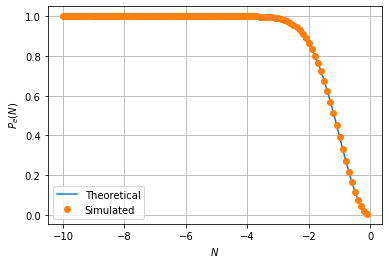
\includegraphics[width=\columnwidth]{7.2.png}
\caption{$P_e(N)$ when A is Rayleigh with scale 1}
\label{fig:probman_p_e}
\end{figure}

%
\item
%
\label{ch4_anal}
For a function $g$,
\begin{equation}
E\sbrak{g(X)} = \int_{-\infty}^{\infty}g(x)p_{X}(x)\, dx
\end{equation}

Find $P_e = E\sbrak{P_e(N)}$.\\
\solution
Since $N \sim \gauss{0}{1}$ ,
\begin{align}
  p_N(x)= \frac{1}{\sqrt{2\pi}}\exp \brak{-\frac{x^2}{2} }\\
\end{align}
And from \eqref{pe(N)} 
\begin{align}
    P_e(x)=
    \begin{cases}
1-\exp\brak{{-\frac{x^2}{2\sigma^2}}} & x<0\\
0 & otherwise
\end{cases}
\end{align}

\begin{align}
 P_e=E\sbrak{P_e(N)} = \int_{-\infty}^{\infty}P_e(x)p_{N}(x)\, dx  
\end{align}
If $x<0, P_e(x)=0$ and using the fact that for an even function
\begin{align}
\int_{-\infty}^{\infty}f(x)=2\int_{-\infty}^{0}f(x)   
\end{align}
we get
\begin{align}
  P_e&= \frac{1}{\sqrt{2\pi}}\int_{-\infty}^{0}\exp \brak{ -\frac{x^2}{2}} \brak{1-\exp \brak{ -\frac{x^2}{2\sigma^2}} }  dx\\
&= \frac{1}{2\sqrt{2\pi}} \int_{-\infty}^{\infty} \exp \brak{ -\frac{x^2}{2} }dx \nonumber \\
&- \frac{1}{2\sqrt{2\pi}} \int_{-\infty}^{\infty} \exp \brak{-\frac{(1+ \sigma^2)x^2}{2 \sigma^2}}  dx\\
&= \frac{\sqrt{2\pi} - \sqrt{\frac{\pi(2\sigma^2)}{1+\sigma^2}}}{2\sqrt{2\pi}}\\
&= \frac{1}{2} - \frac{1}{2}\sqrt{\frac{\sigma^2}{1+\sigma^2}}
\end{align}
For a Rayleigh Distribution with scale $= \sigma$,
\begin{align}
E\sbrak{A^2} = 2\sigma^2\\
\gamma = 2\sigma^2\\
\therefore P_e = \frac{1}{2} - \frac{1}{2}\sqrt{\frac{\gamma}{2+\gamma}}
\end{align}
%
\item
Plot $P_e$ in problems \ref{ch4_sim} and \ref{ch4_anal} on the same graph w.r.t $\gamma$.  Comment.

%
\end{enumerate}
\end{document}
